\documentclass[./project-report/src/latex/project-report.tex]{subfiles}

\begin{document}

\maketitle

\clearpage

\section{Investigation}

This section outlines the code utilised to test the performance of a trained network. It then utilises this functionality to explore the effects of Hyper-Parameters on the 
Artificial Neural Network performance.

\subsection{test\_model module}
\label{sec:test_model-module}

The test\_model module is contained within the frames package, and contains tkinter frames for testing the trained Artificial Neural Network models for each dataset. 
For each training dataset that an Artificial Neural Network is trained on, there is a corresponding test dataset with completely new images to be tested on to judge 
the performance of the trained model. As fewer images are needed for testing than for training, the Cat dataset only has 50 test images (compared to the 209 images 
for training) and the MNIST dataset only has 10,000 test images (compared to the 60,000 images for training).
Each frame displays the results of the testing along with a random selection of incorrect and correct predictions.

\inputminted{python}{./school_project/frames/test_model.py}

Which outputs the following for the MNIST dataset:

\pagebreak

\begin{figure}[h!]
\centering
\frame{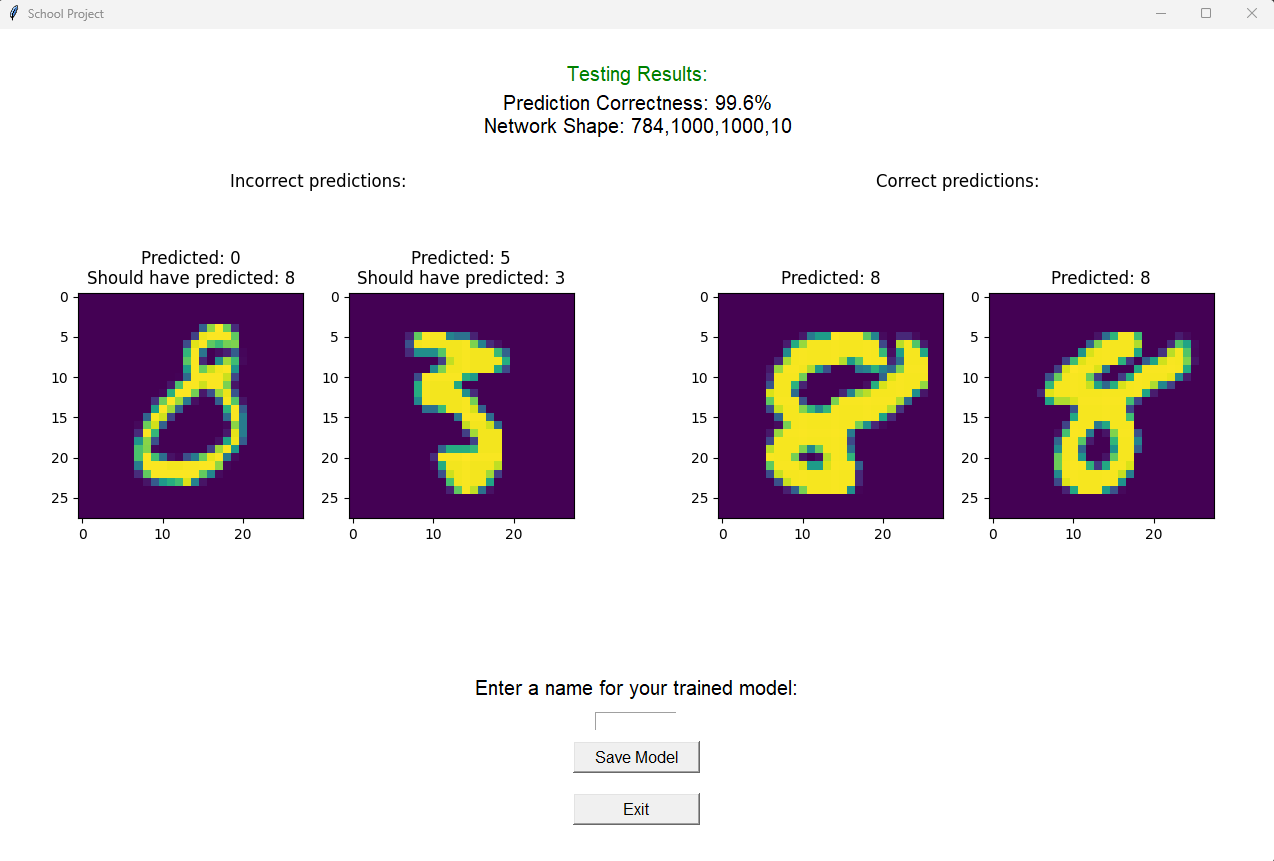
\includegraphics[width=1\textwidth]{./project-report/src/images/test-mnist-frame.png}}
\caption{Model test results for MNIST database}
\label{fig:test-frame-impl}
\end{figure}

And outputs the following for the Cat Recognition dataset:

\pagebreak

\begin{figure}[h!]
\centering
\frame{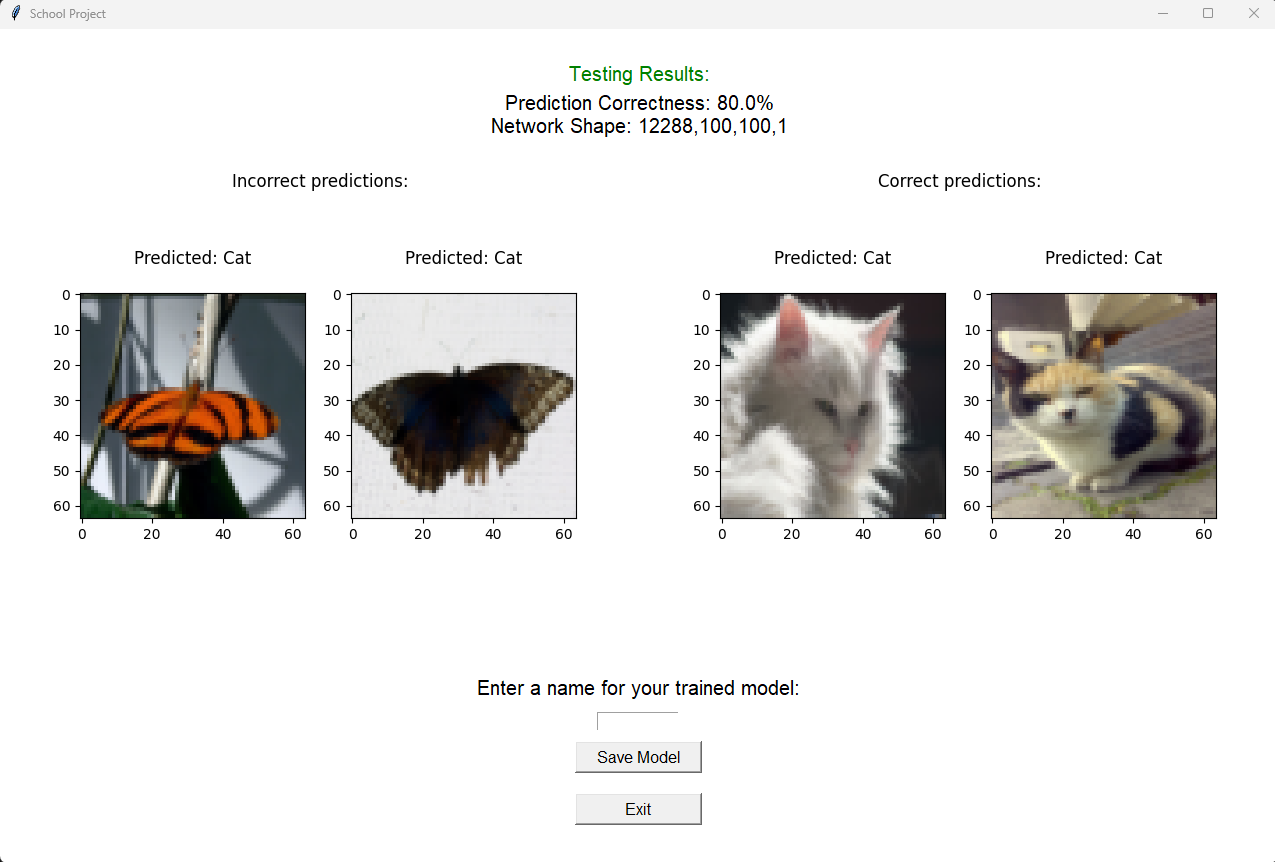
\includegraphics[width=1\textwidth]{./project-report/src/images/test-cat-recognition-frame.png}}
\caption{Model test results for Cat recognition database}
\end{figure}

And outputs the following for the XOR dataset:

\pagebreak

\begin{figure}[h!]
\centering
\frame{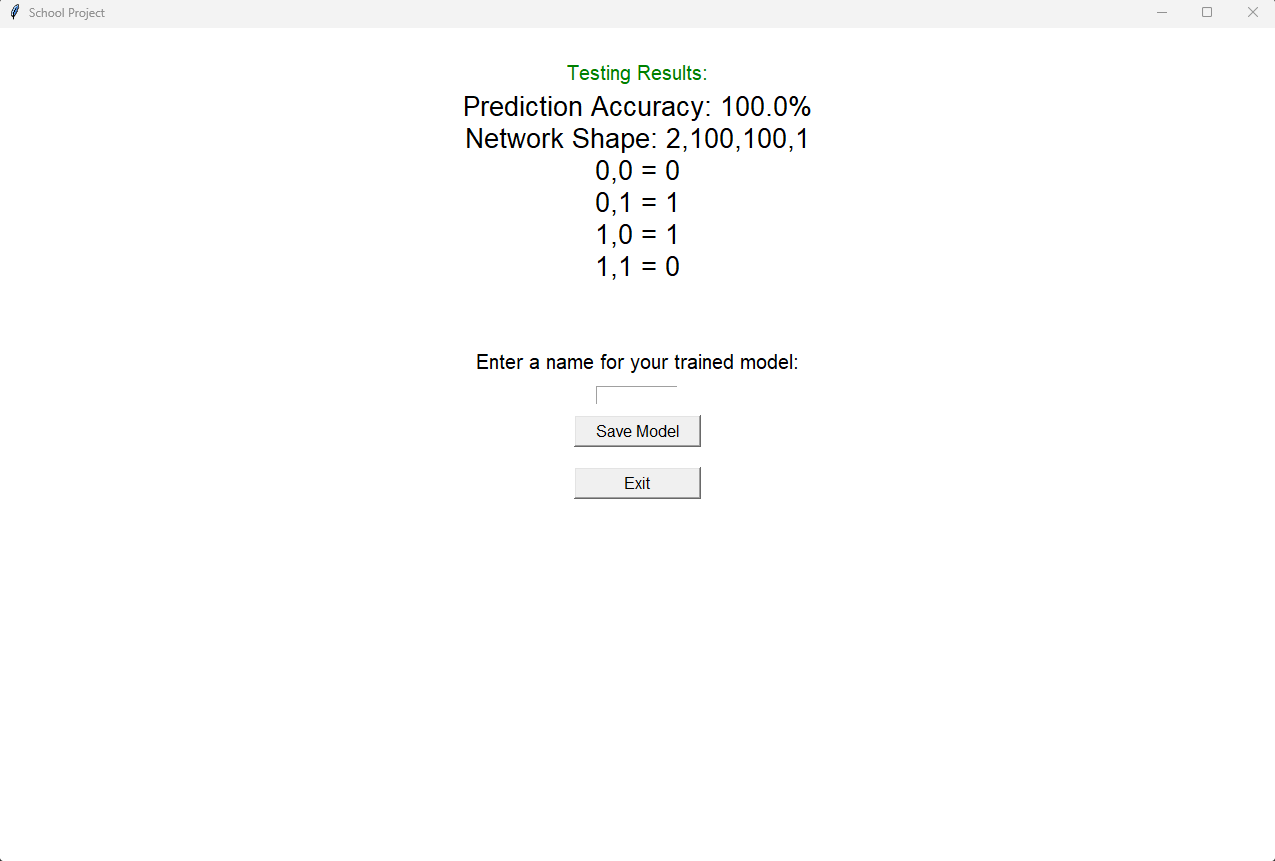
\includegraphics[width=1\textwidth]{./project-report/src/images/test-xor-frame.png}}
\caption{Model test results for XOR dataset}
\end{figure}

\subsection{Effects of Hyper-Parameters}
\label{sec:effects-of-hyper-parameters}

For the following investigations, I utilised Jupyter Notebook and have displayed the results below:

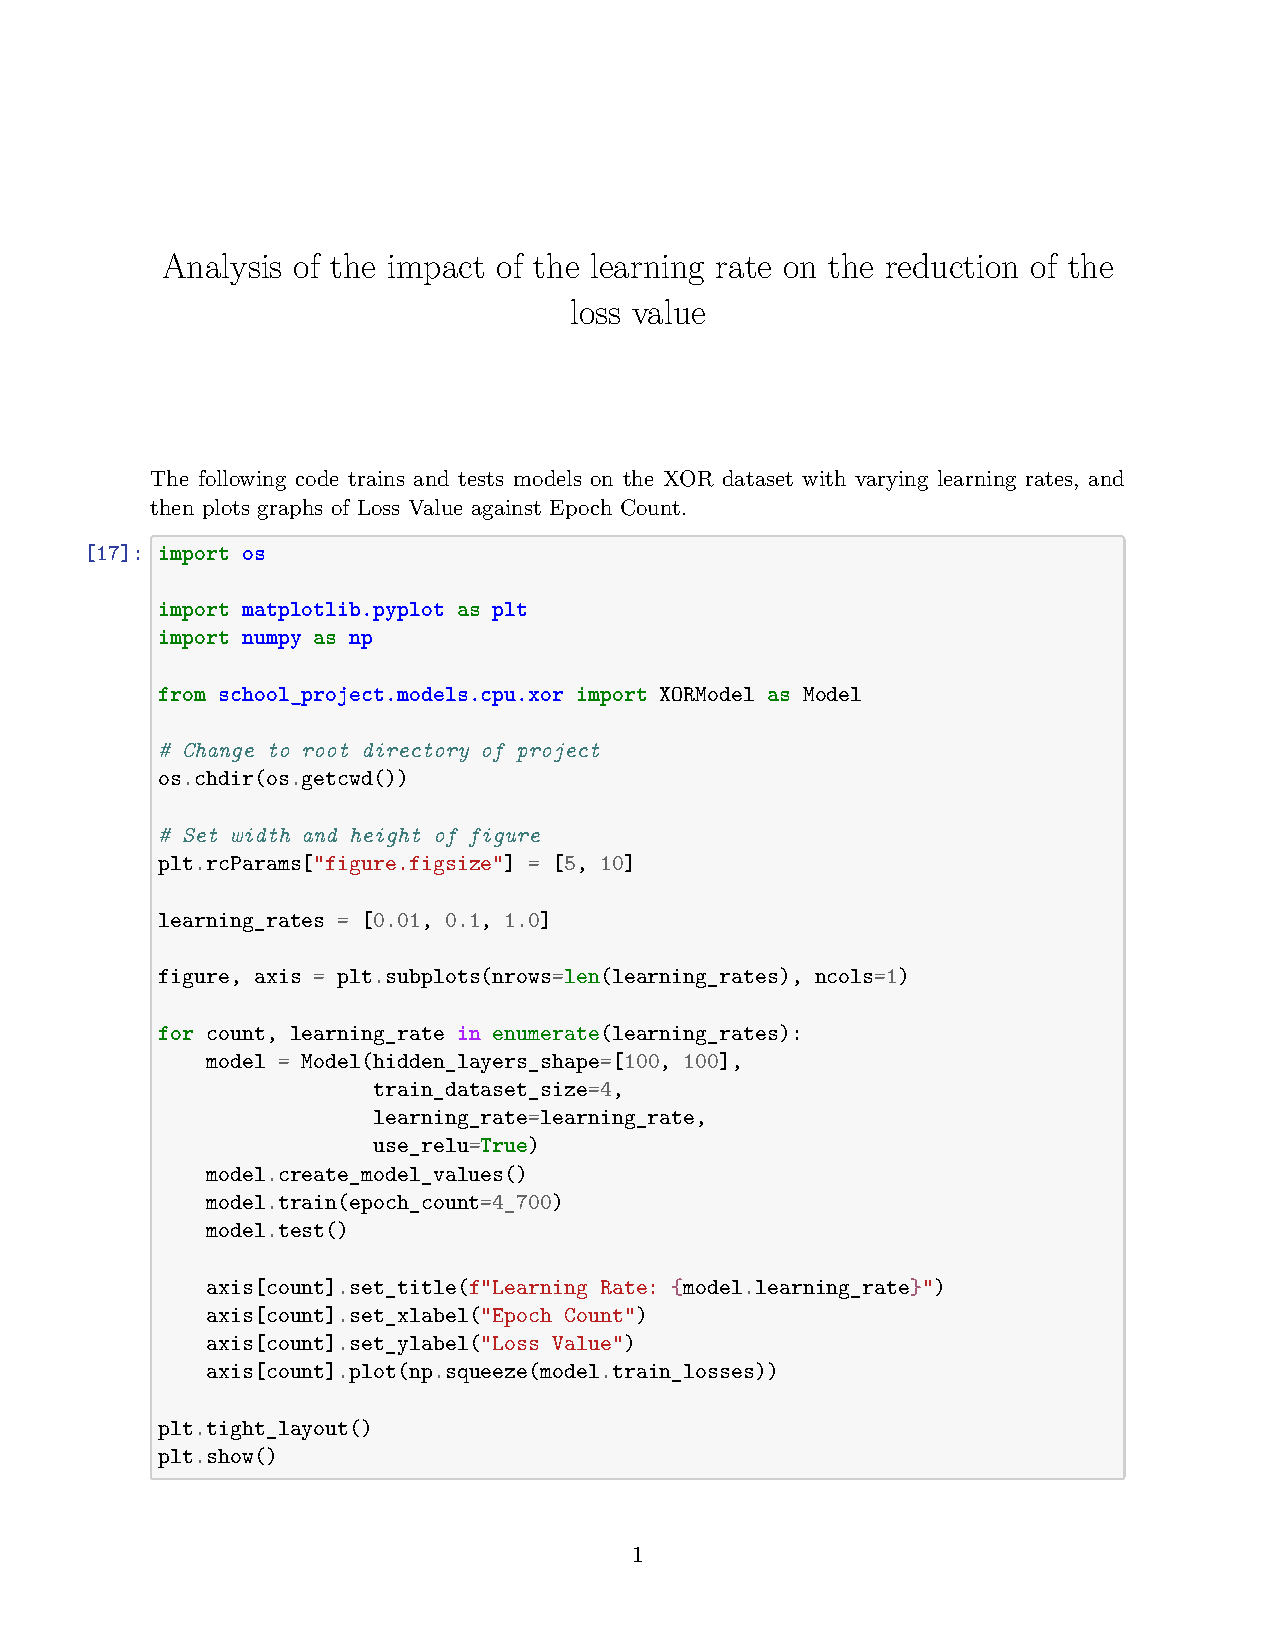
\includepdf[pages=-, pagecommand={\thispagestyle{plain}}, scale=0.9]{./project-report/src/pdfs/learning-rate-analysis.pdf}
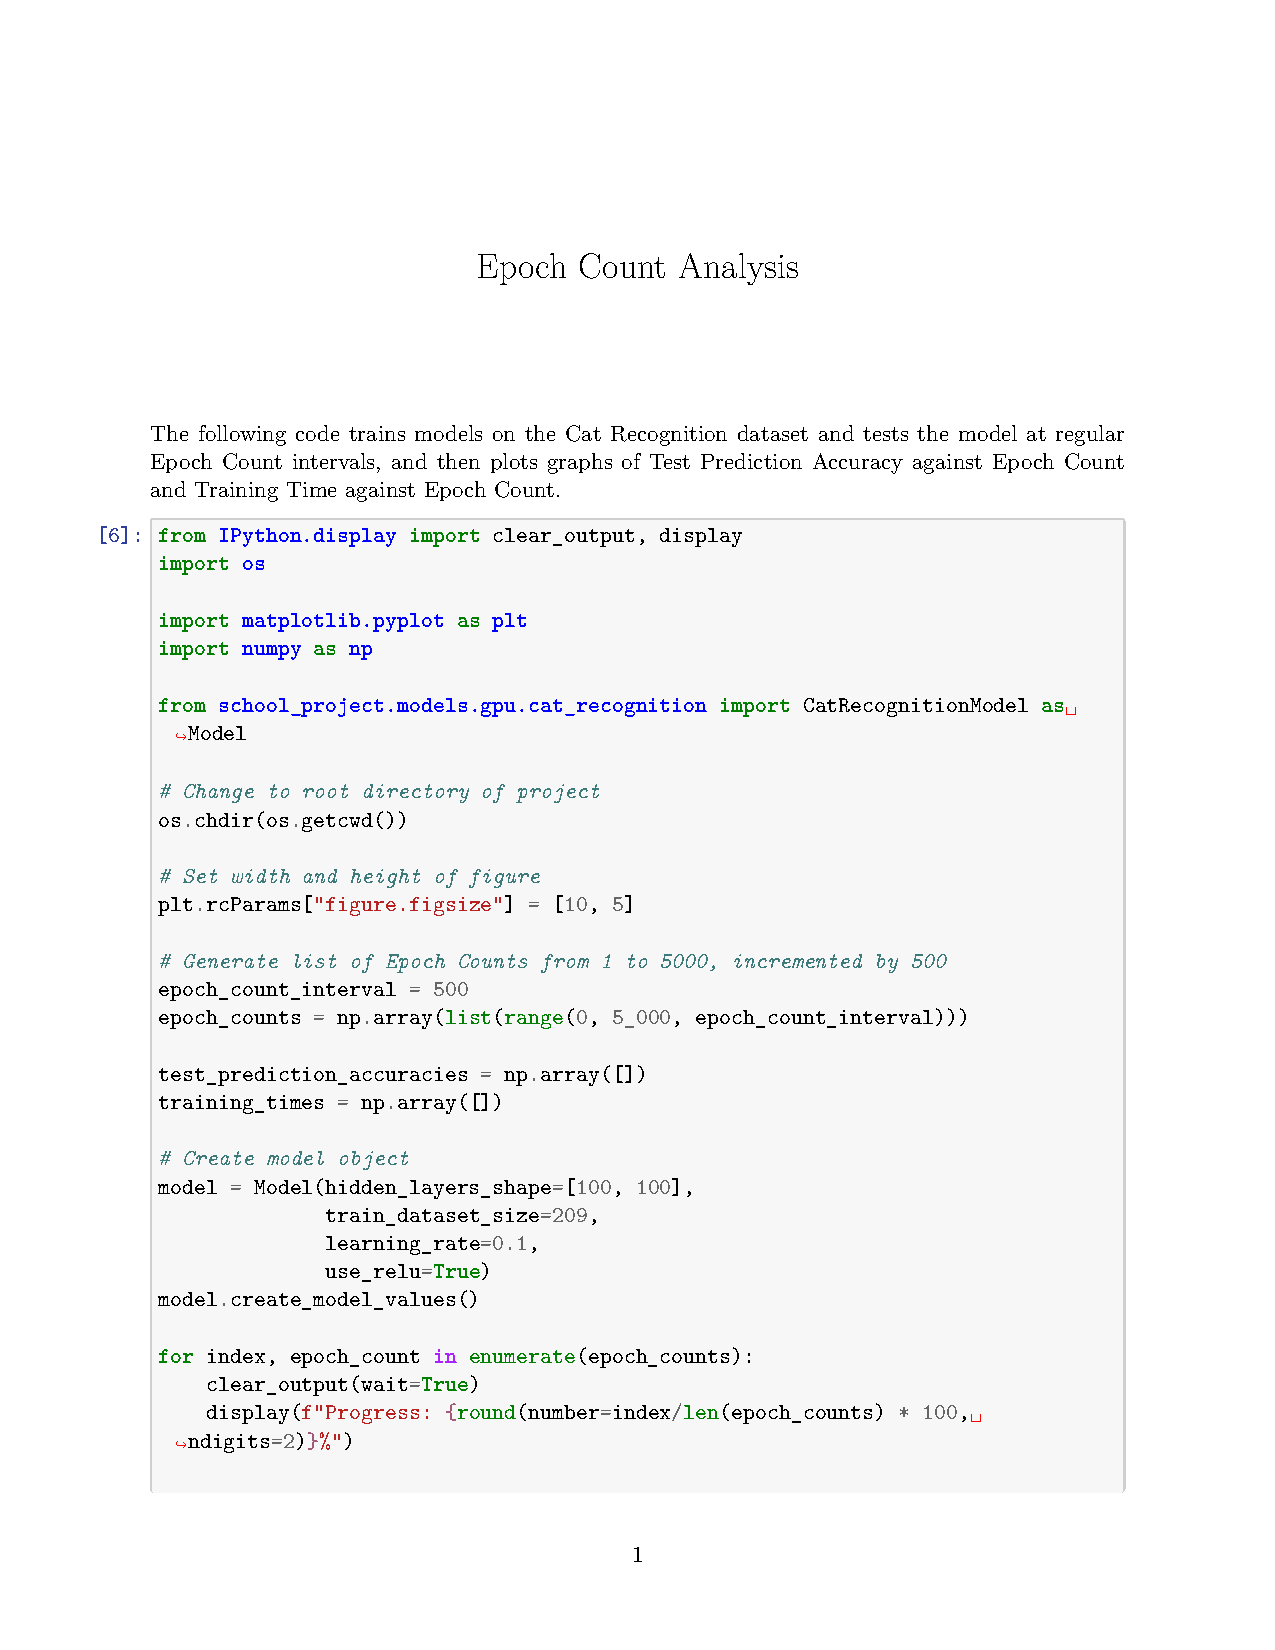
\includepdf[pages=-, pagecommand={\thispagestyle{plain}}, scale=0.9]{./project-report/src/pdfs/epoch-count-analysis.pdf}
\label{sec:train-dataset-size-analysis}
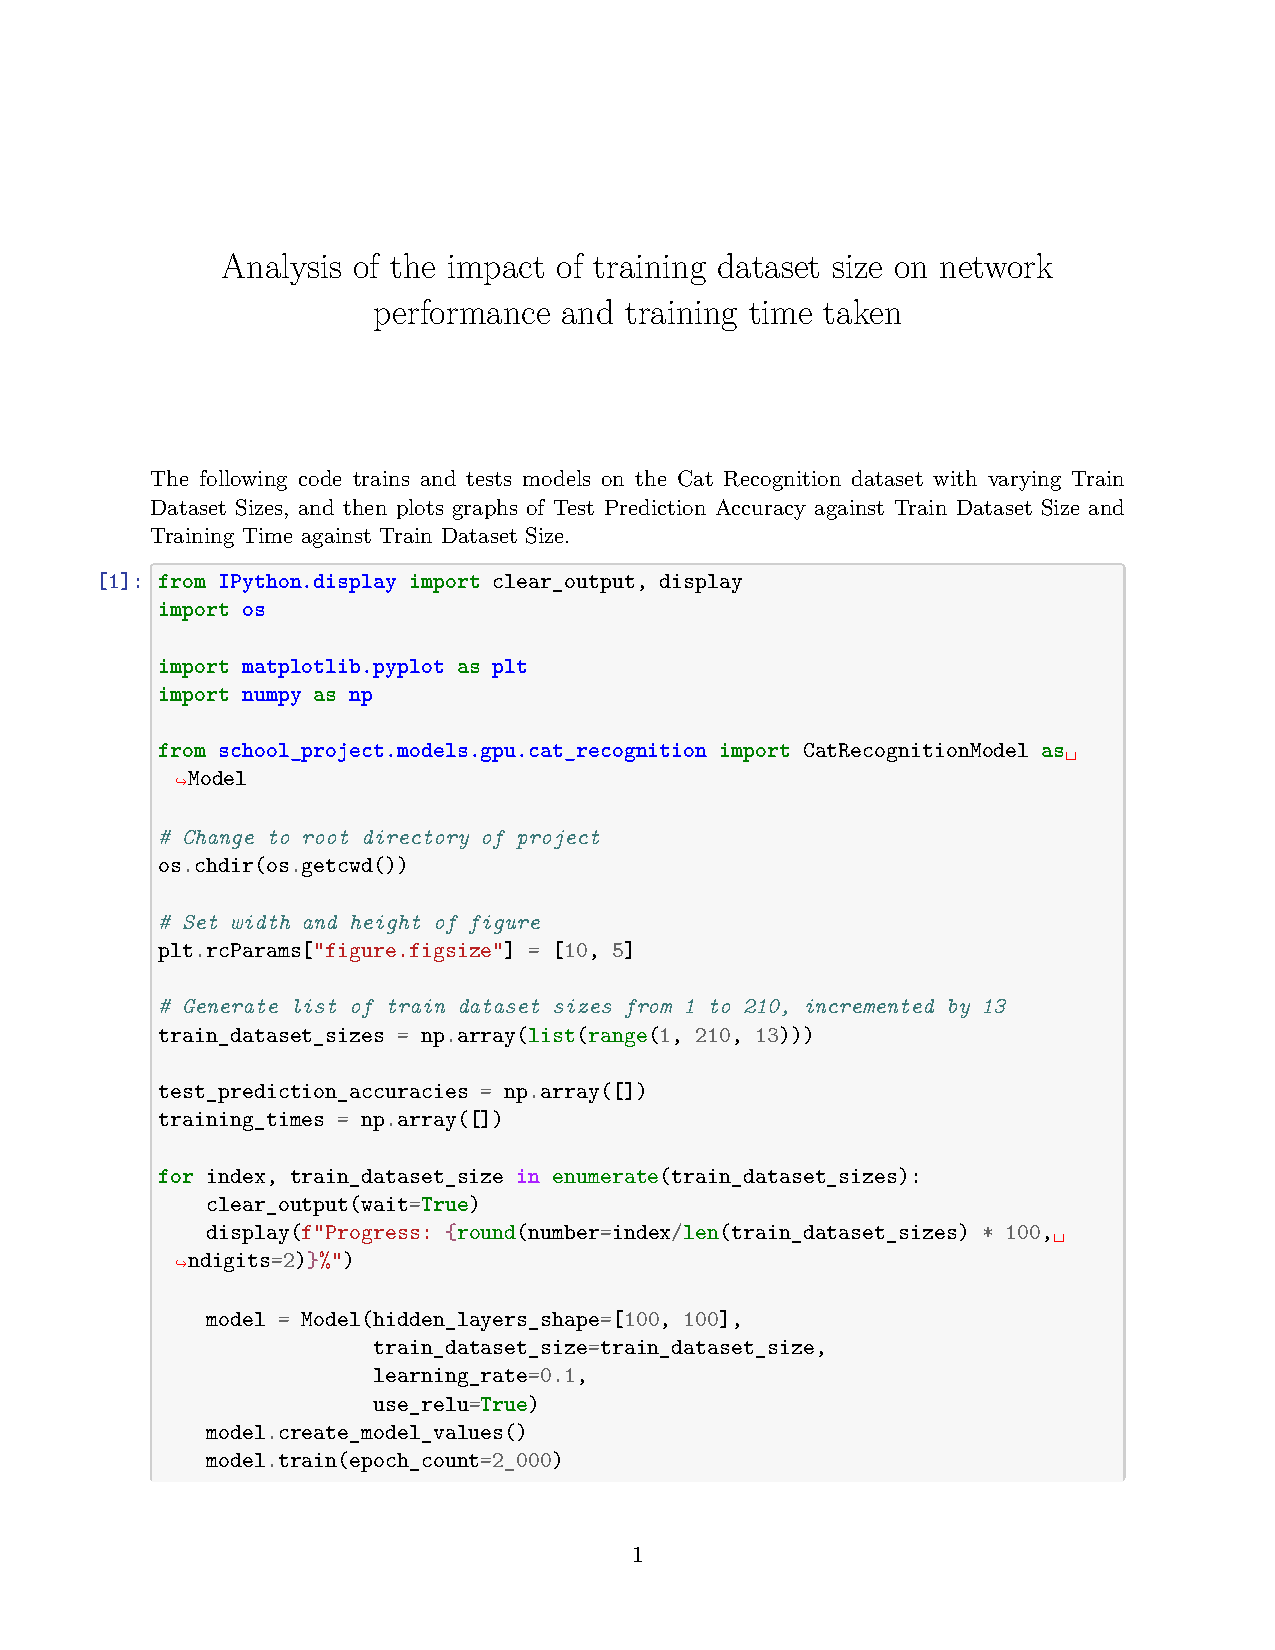
\includepdf[pages=-, pagecommand={\thispagestyle{plain}}, scale=0.9]{./project-report/src/pdfs/train-dataset-size-analysis.pdf}
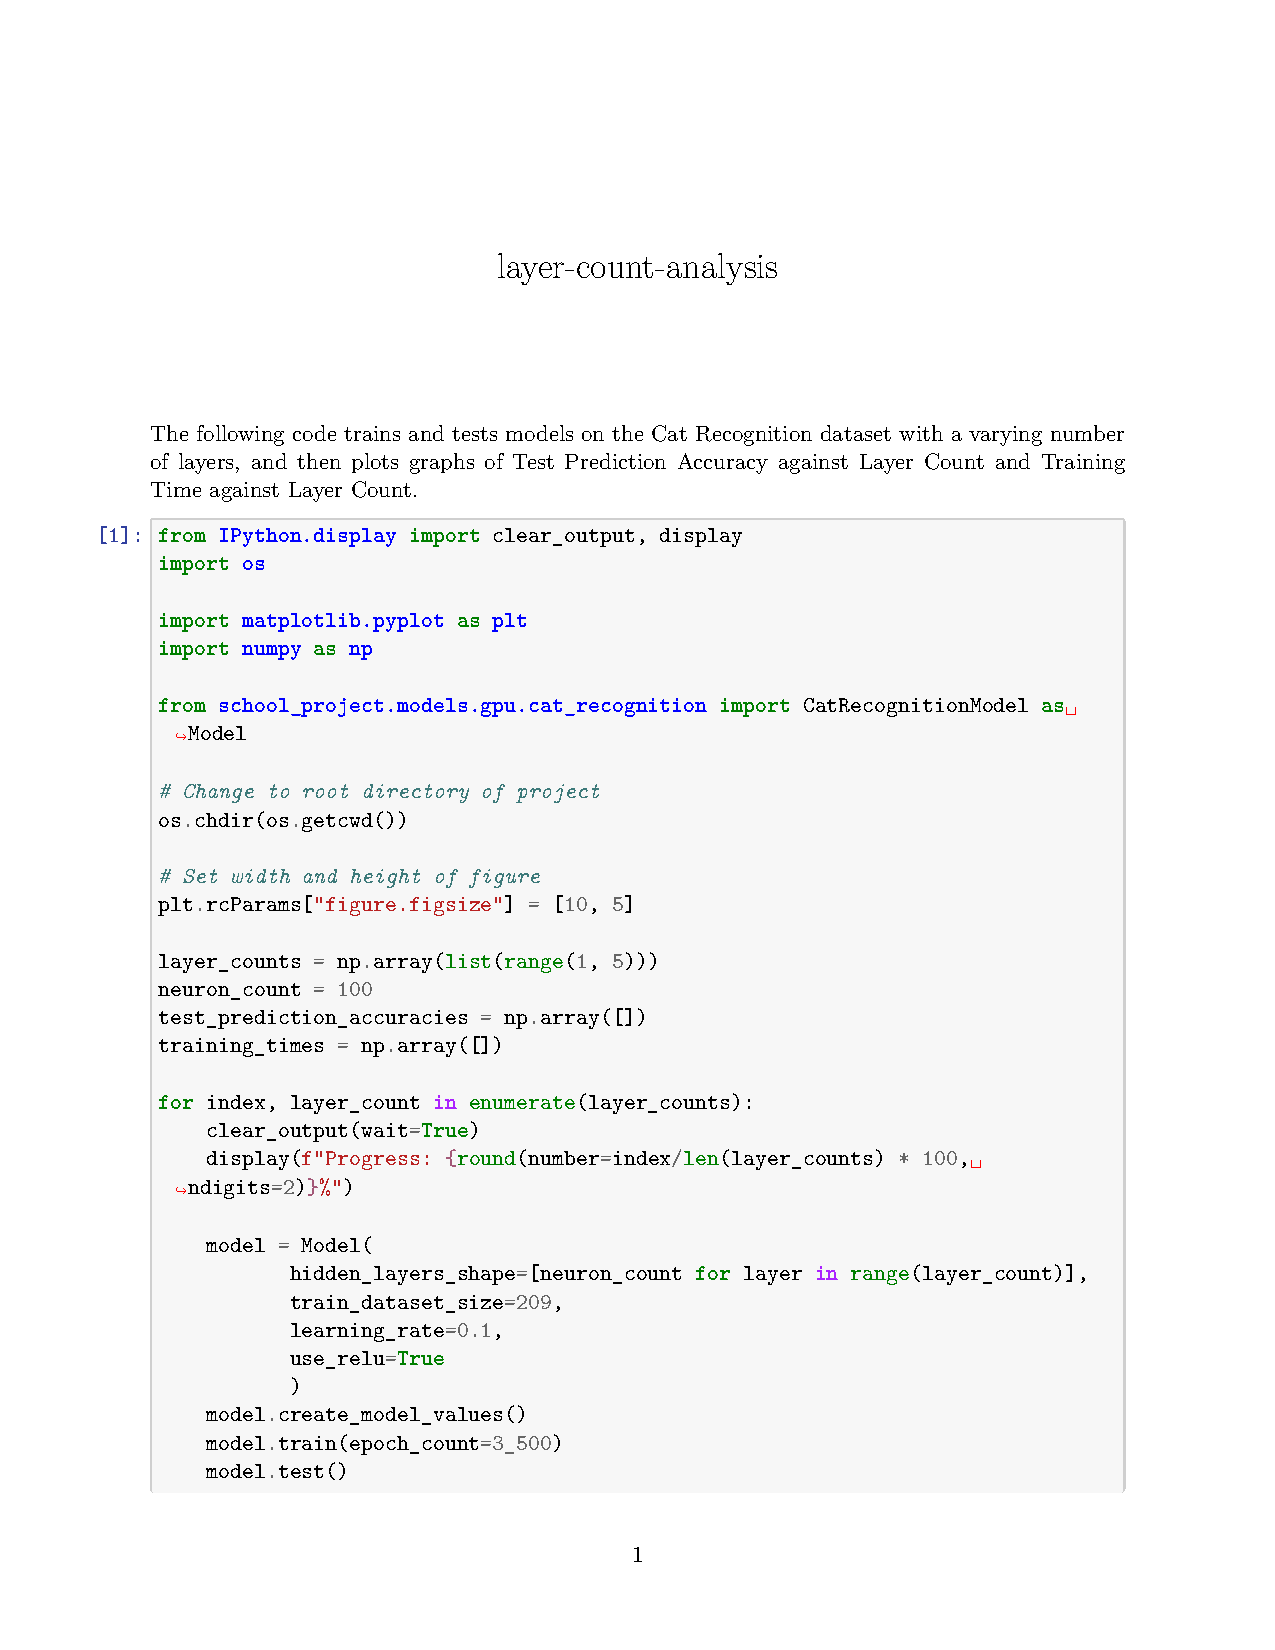
\includepdf[pages=-, pagecommand={\thispagestyle{plain}}, scale=0.9]{./project-report/src/pdfs/layer-count-analysis.pdf}
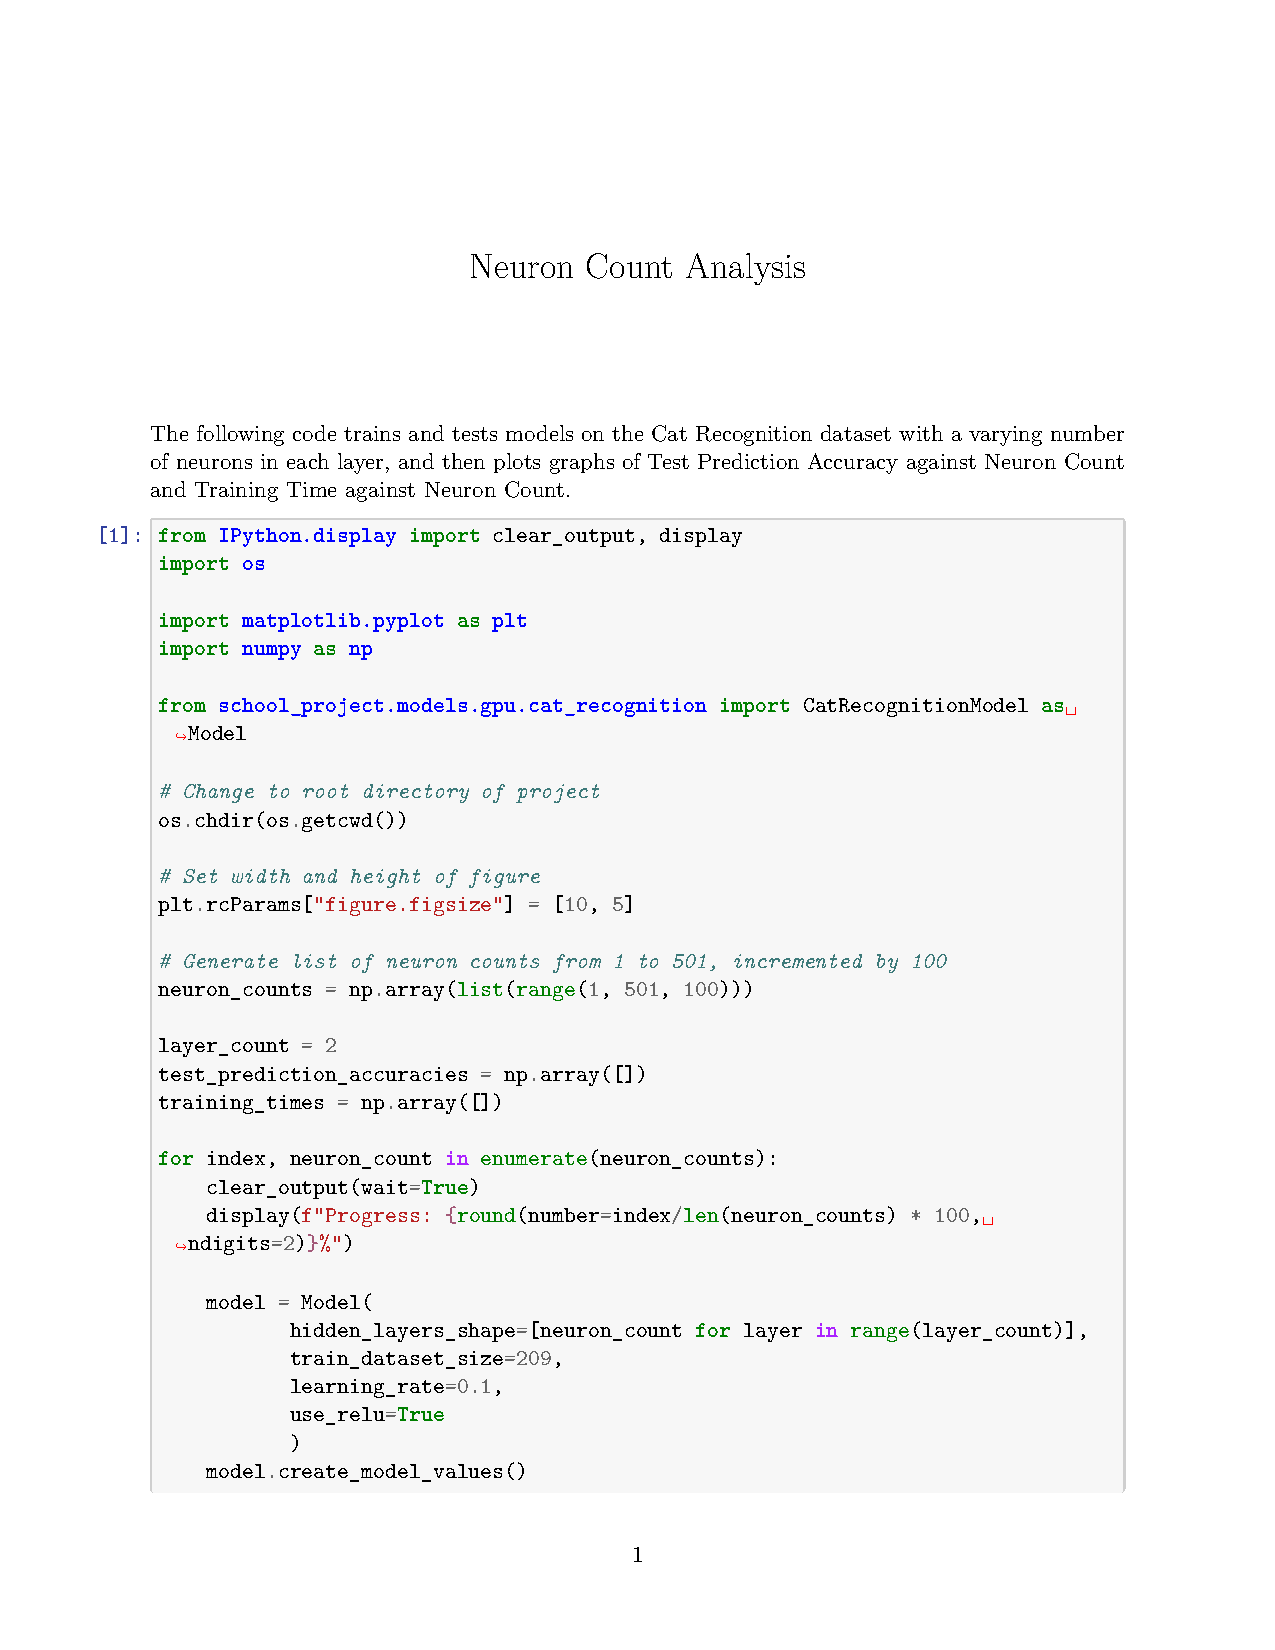
\includepdf[pages=-, pagecommand={\thispagestyle{plain}}, scale=0.9]{./project-report/src/pdfs/neuron-count-analysis.pdf}
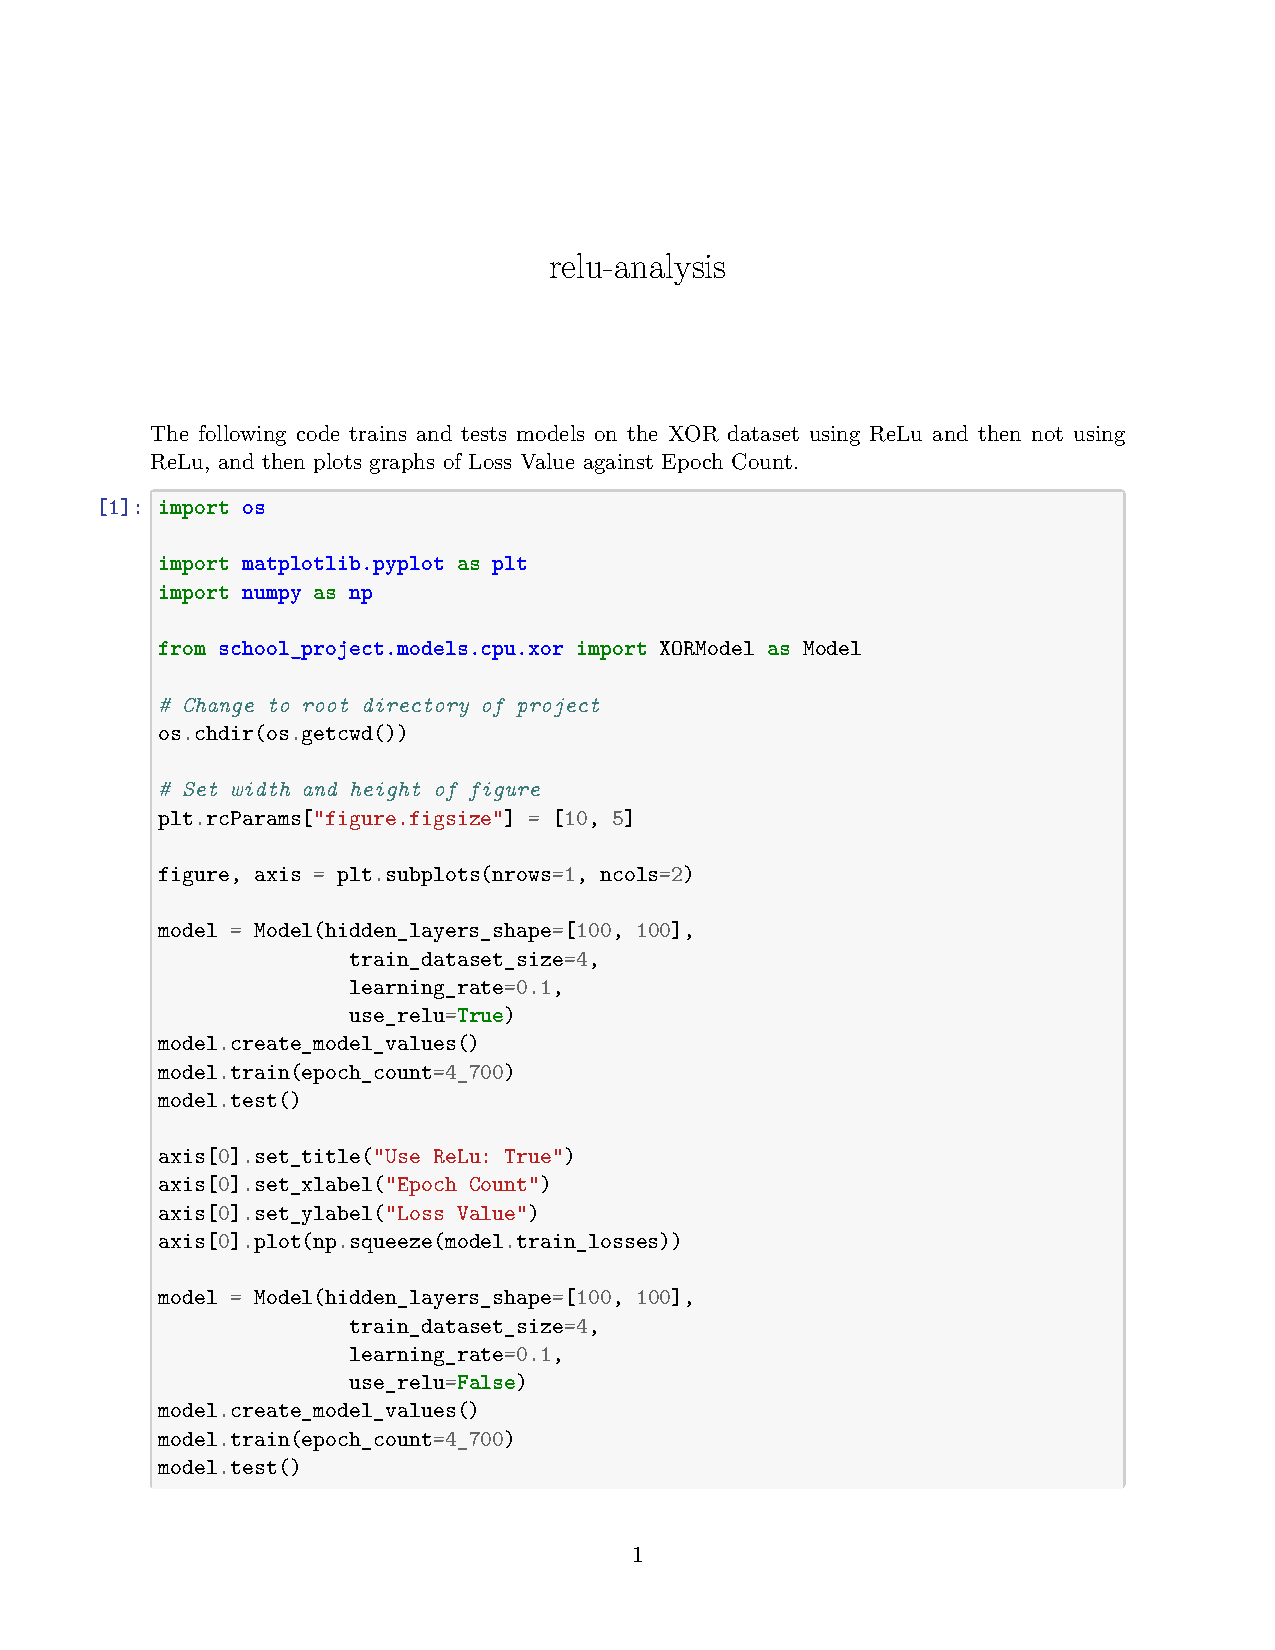
\includepdf[pages=-, pagecommand={\thispagestyle{plain}}, scale=0.9]{./project-report/src/pdfs/relu-analysis.pdf}
\label{sec:cpu-vs-gpu-analysis}
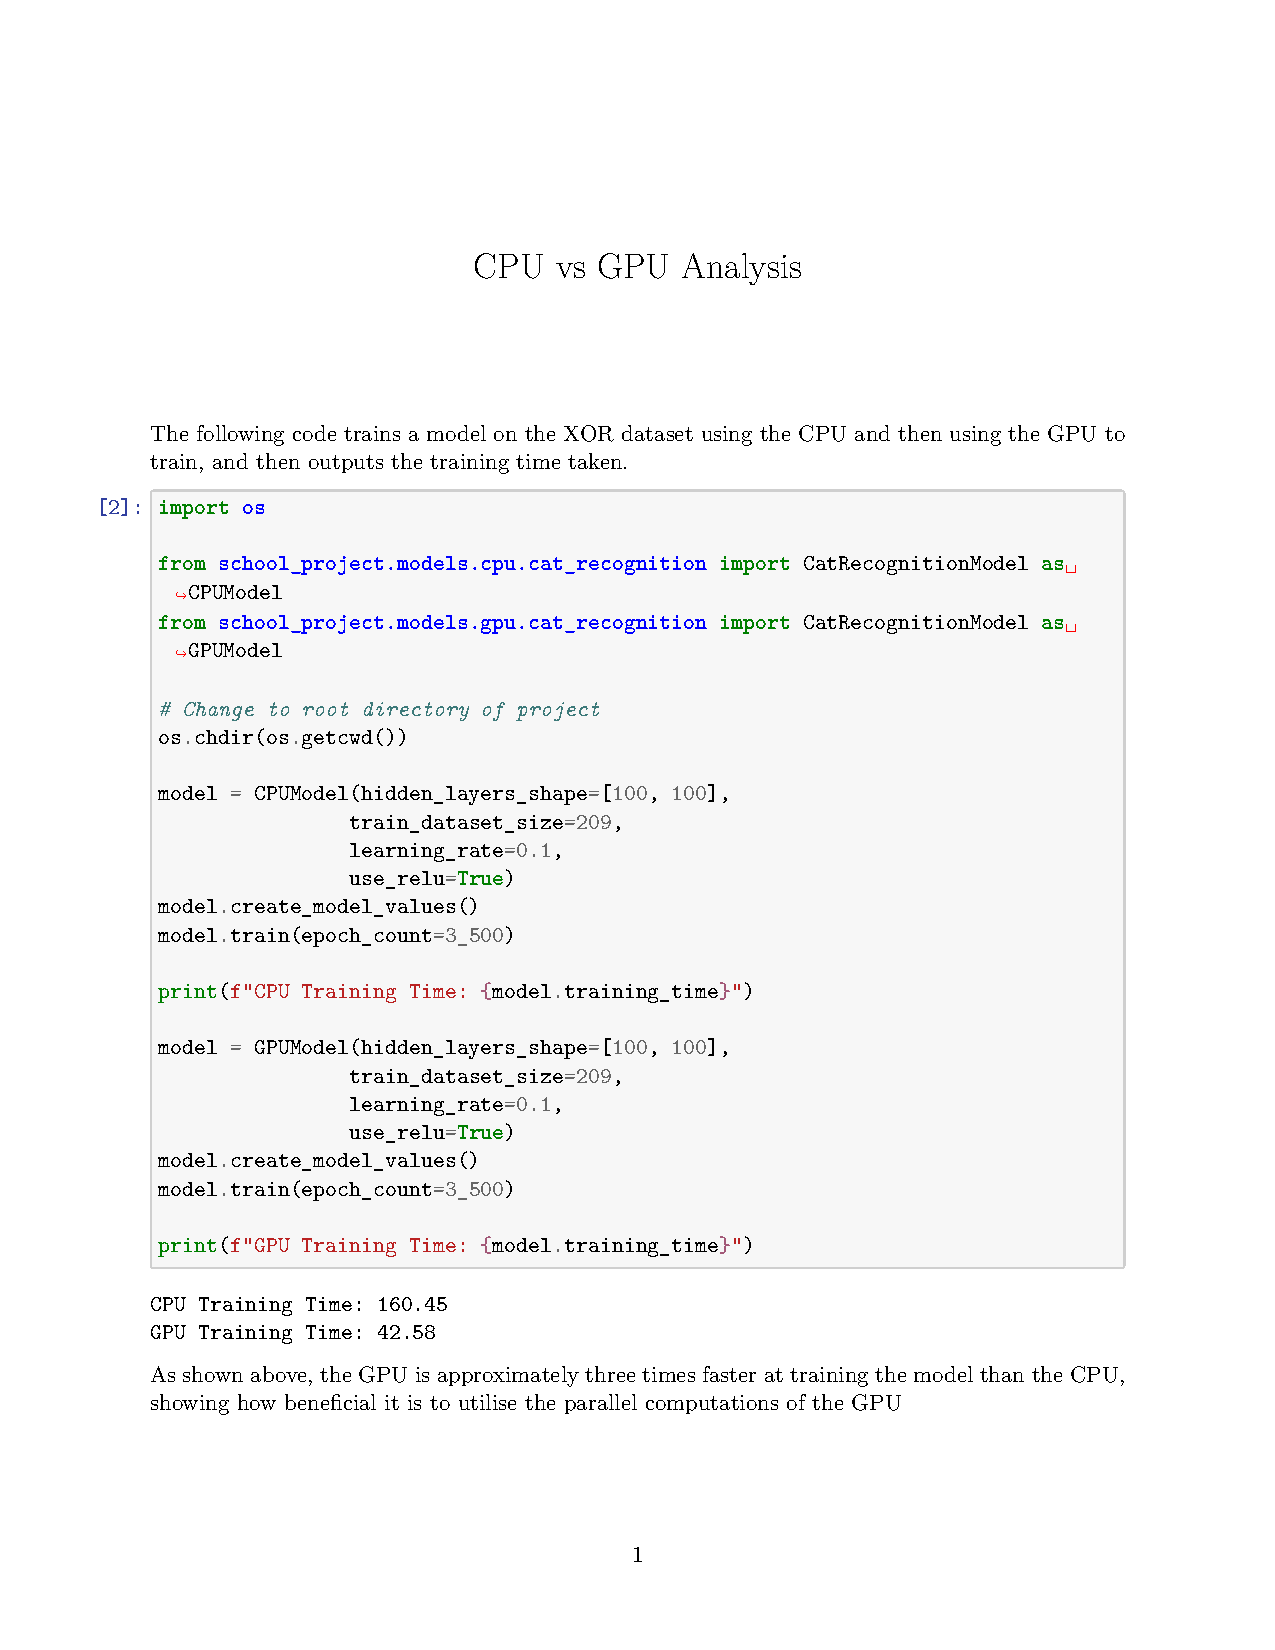
\includepdf[pages=-, pagecommand={\thispagestyle{plain}}, scale=0.9]{./project-report/src/pdfs/cpu-vs-gpu-analysis.pdf}

\pagebreak

\end{document}
